
%!TEX ROOT=main.tex


\part{Results}
\label{chap:results}
\section{Overall}
The built RC system was successfully tested in real-life conditions. The car behaves as expected from an RC car. The connection between the transmitter and the car is quickly established, even though the antenna is usually hidden under the plastic shell. The driving works flawlessly; the control is responsive and smooth. Trimming encoders can correct any misbehavior, for example, small steering to one side.

Suppose the signal is lost and no command arrives in \SI{250}{\ms} from the last one. In that case, the dedicated safety-timer resets actuators to their neutral position. The vehicle comes to a slow stop and waits until another command packet is successfully received.

Extra features such as OLED status display with interactive indicators also work as expected and wirelessly provide the user with additional information about the RC car.

Data logging to the SD card is operational, too, making it possible to record driving data and analyze them afterward. An example of the graphed output data is in the section below in figure \ref{fig:sd_speed}.

The battery life was not measured as it depends on a lot of factors. However, during the testing, the car was able to drive for about an hour. The battery life of the transmitter could not even be estimated because the battery hardly needed to be charged.

Furthermore, two experiments were realized to obtain maximum speed and communication range.

\section{Speed}
The car's maximum speed was tested in Ladronka park on a flat asphalt cycle path. The speed was measured by GPS and consisted of three test runs. An Honor 9 smartphone running GPS speedometer app DigiHUD was taped to the chassis. Before each run, the app's statistics were reset.

The car accelerated quickly and drove in a straight line with the full throttle until it stopped accelerating visually. Then the throttle was released, and the car performed a U-turn and began accelerating again. This process was repeated at least two times in each run.

Data logging to the SD card was enabled for all three test runs to monitor battery voltage, as the motor's maximum speed depends on its supply voltage. Measured data from the last run are graphed in figure \ref{fig:sd_speed}. The test scheme described above is clearly visible - negative peaks in \textit{'STEER'} data paired with positive peaks in \textit{'GYRO\_Z'} data represent U-turns; saturated \textit{'THRTL'} with \textit{'VOLTAGE'} drops and \textit{'CURRENT'} peaks represent straight-line accelerations.
\begin{figure}[h]
\centering
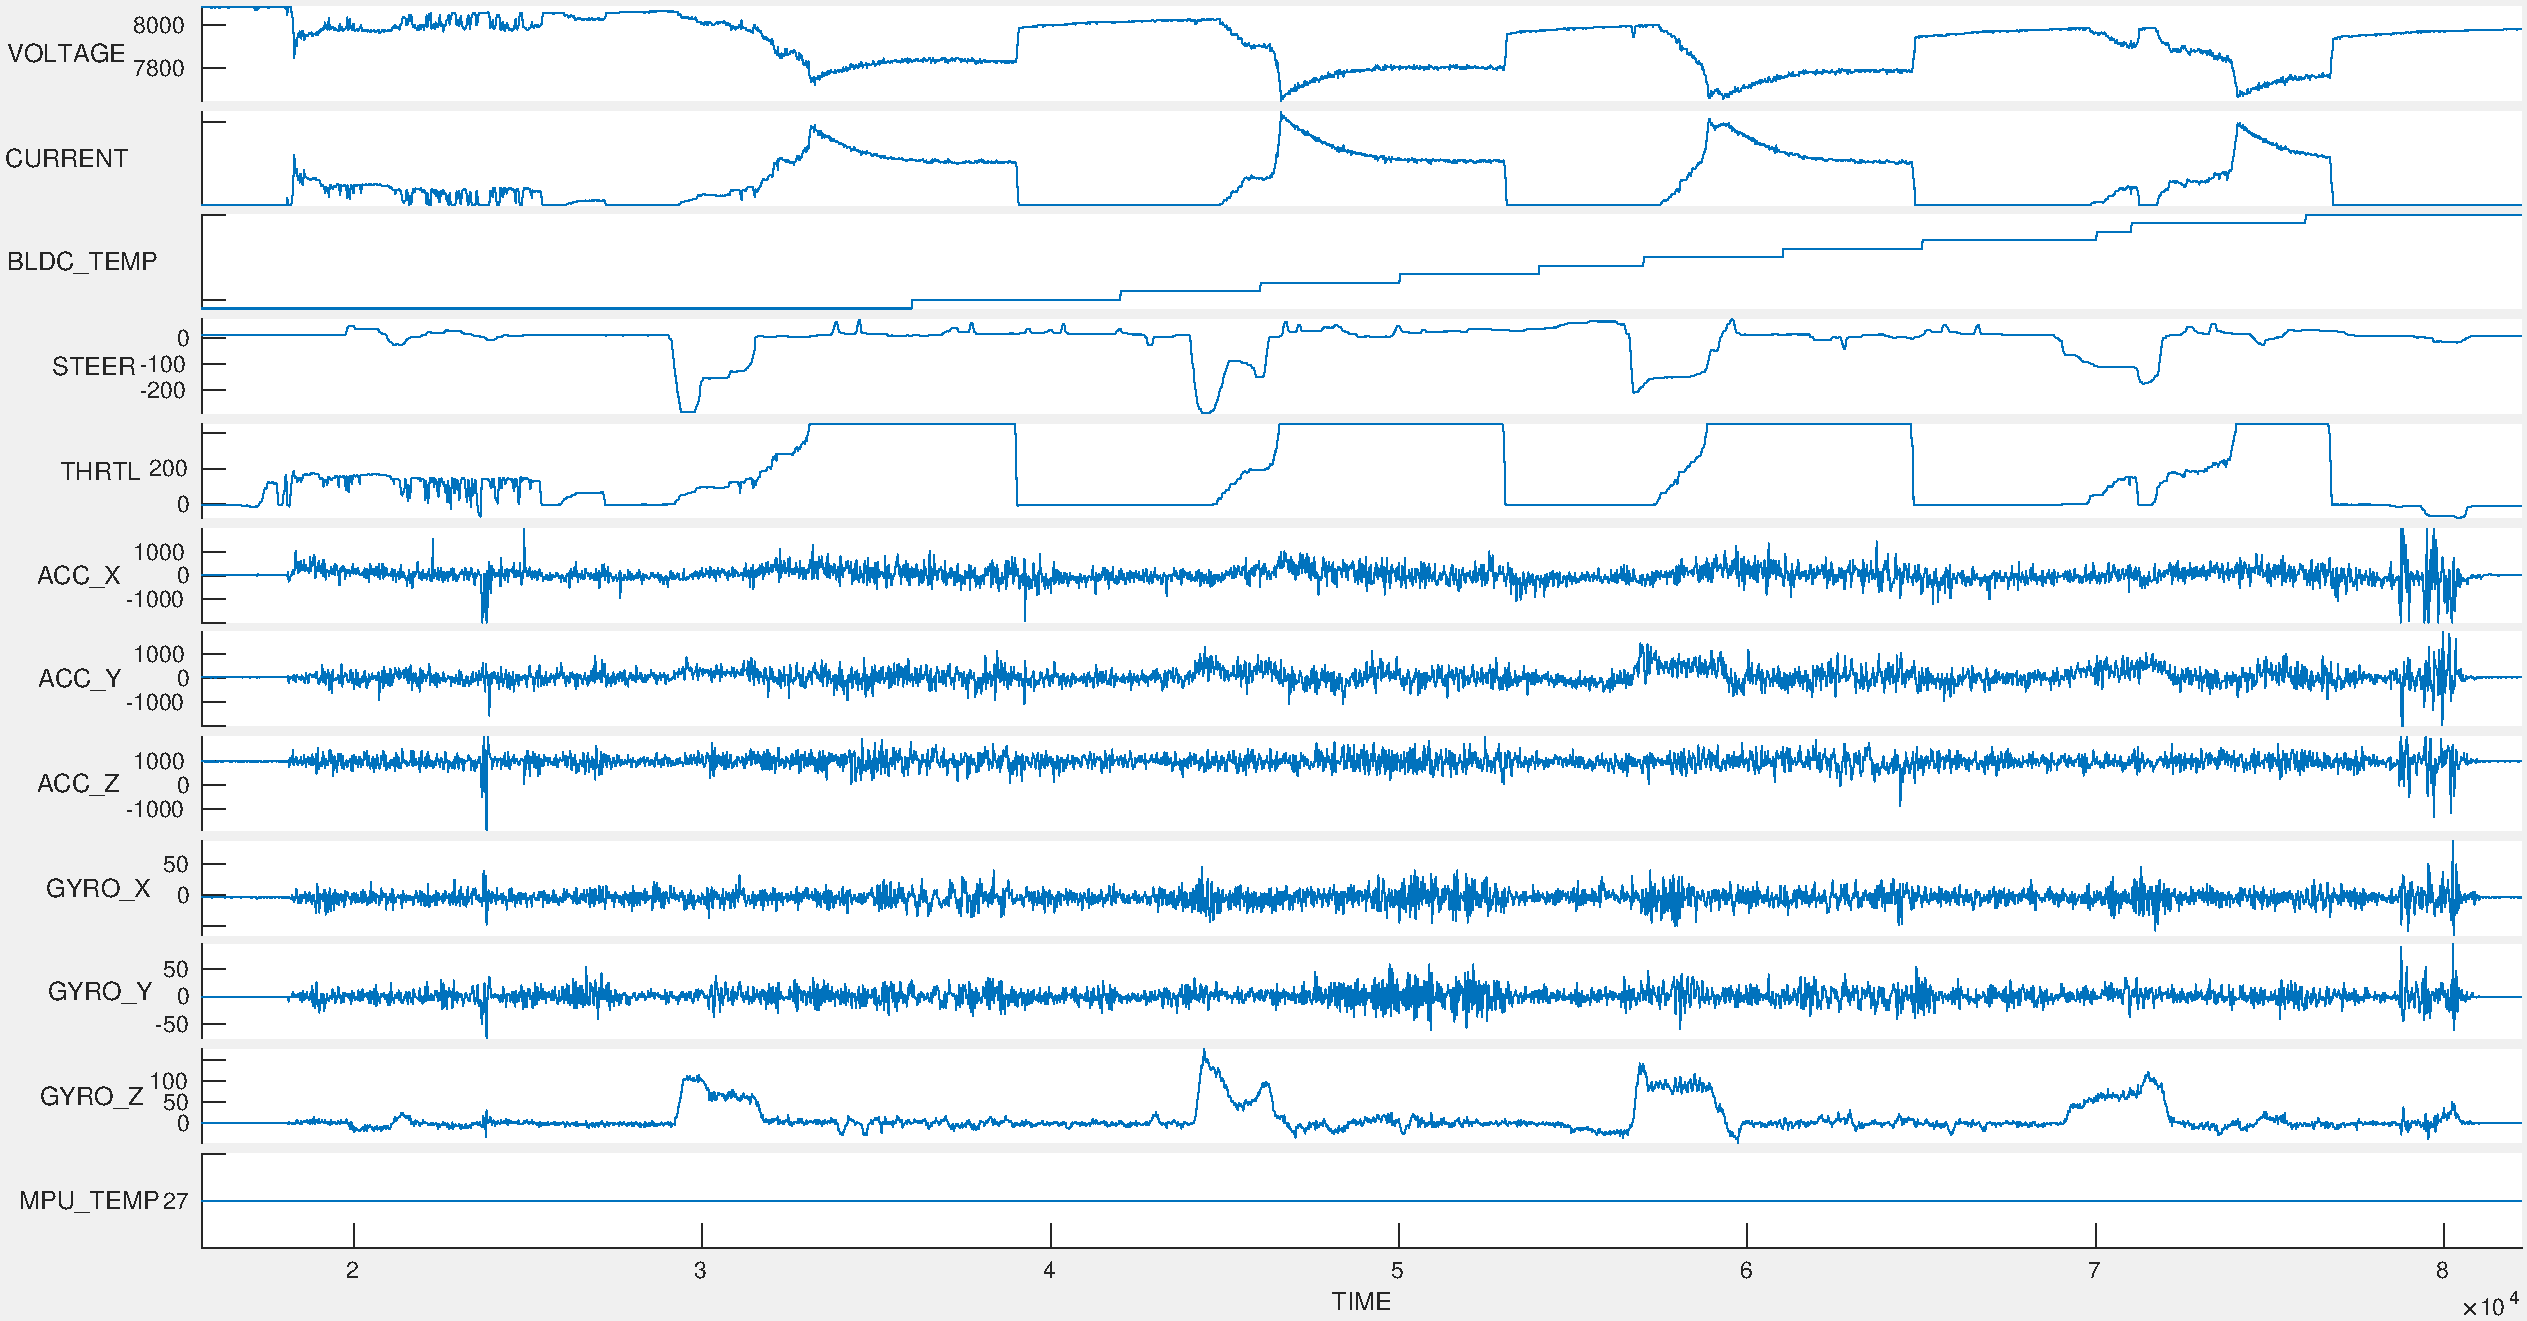
\includegraphics[width=1\linewidth]{fig/run3.pdf}
\caption{Data from last speed-test run}
\label{fig:sd_speed}
\end{figure}

Although the battery voltage dropped by approximately \SI{0.1}{\V} between runs, during all three of them, the car reached a maximum speed of \SI{35}{\km\per\hour}. Photos of the results of the runs are shown in figure \ref{fig:speed}.
\begin{figure}[h]
    \centering
    \begin{subfigure}{0.3\textwidth}
    \centering
        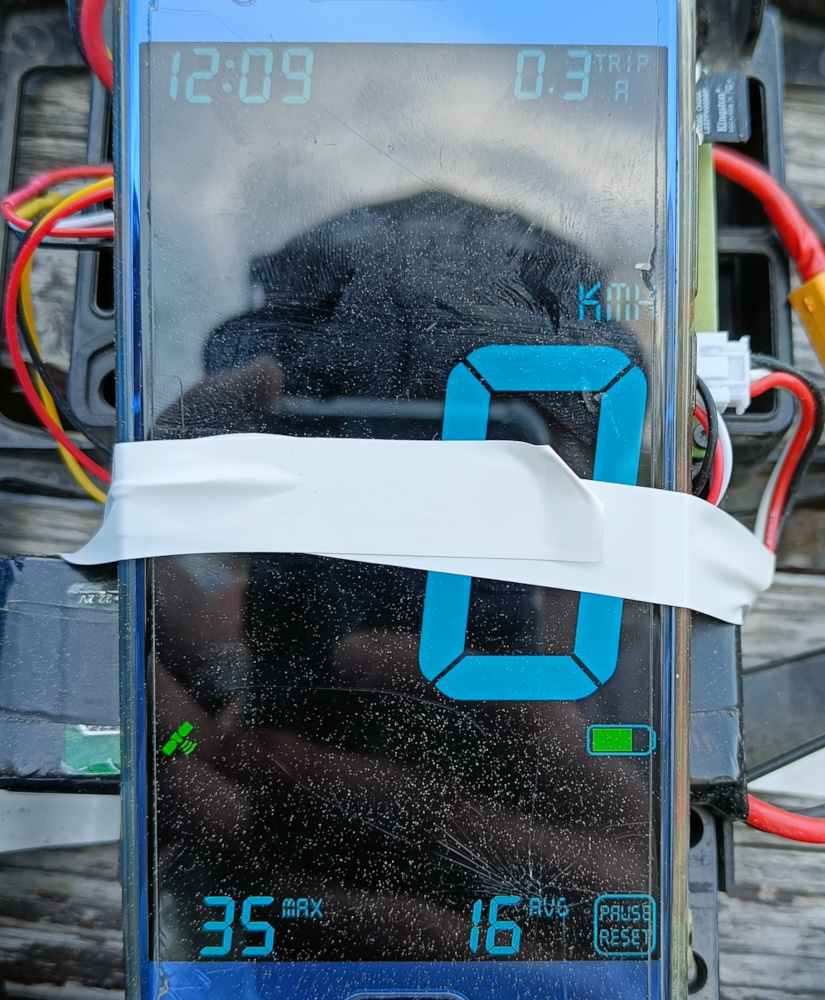
\includegraphics[width=1\textwidth]{fig/speed_run1.jpg}
		\caption{test run 1}
    \end{subfigure}%
    \hspace{0.2cm}
    \begin{subfigure}{0.3\textwidth}
    \centering
		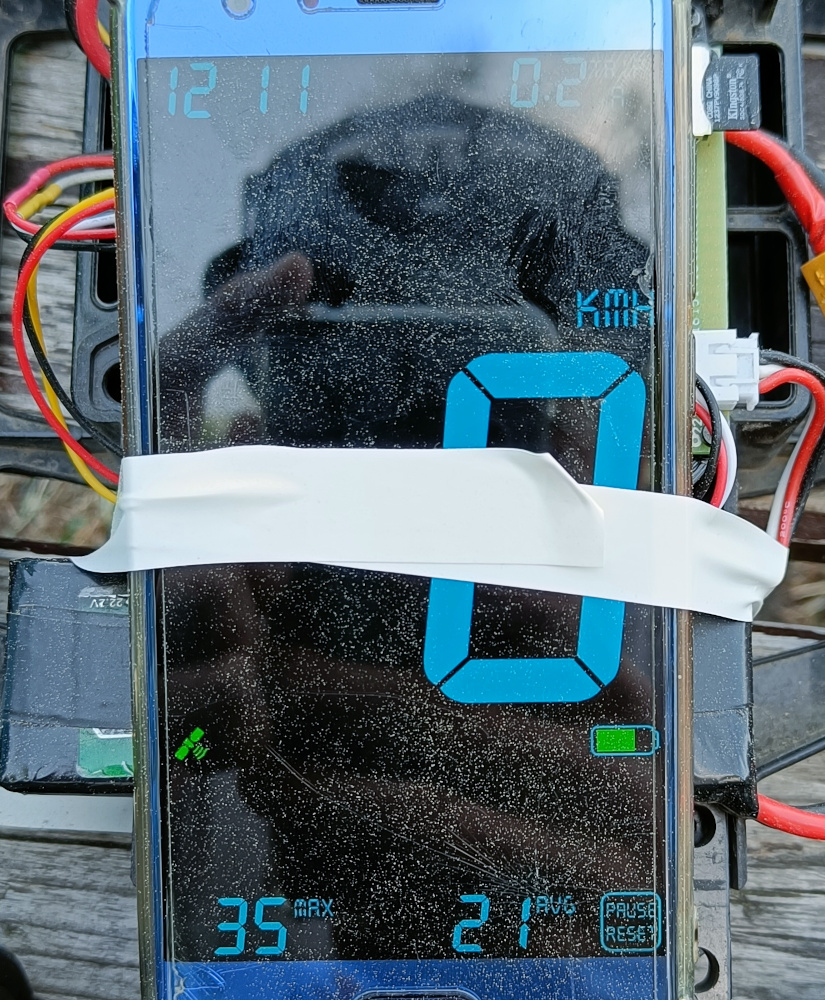
\includegraphics[width=1\textwidth]{fig/speed_run2.jpg}
		\caption{test run 2}
    \end{subfigure}
    \hspace{0.2cm}
    \begin{subfigure}{0.3\textwidth}
    \centering
		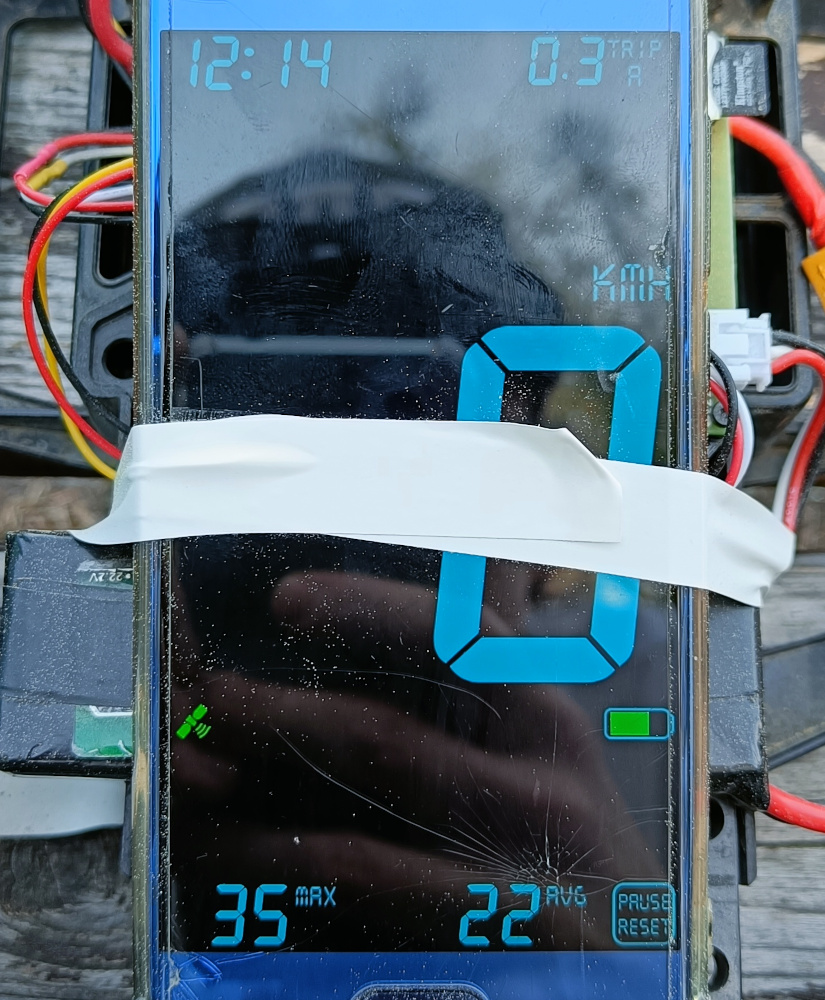
\includegraphics[width=1\textwidth]{fig/speed_run3.jpg}
		\caption{test run 3}
    \end{subfigure}
	\caption{Results of the speed test}
    \label{fig:speed}
\end{figure}

\section{Range}
The range test was also performed in Ladronka park. The test is mainly informative since the car is barely visible at about \SI{250}{\m}. The expected maximum range given by used communication modules was \SI{800}{\m}; therefore, the distance was calculated from GPS coordinates.

The test utilized the vehicle's signal loss detection feature. The transmitter was configured to send the steering command to keep the front wheels turned. The signal loss was easily recognizable since the signal loss detection feature resets the motor and straightens the servo. Both antennas were in a vertical position during the test for the best signal reception.

First, coordinates of the transmitter's initial position were acquired. Then the chassis was moved in a straight direction to keep the transmitter in sight until the signal began to fade.

After \SI{375}{\m}, the servo started to straighten occasionally, indicating that no command packet was received within \SI{250}{\ms} from the last one. Even though the safety-timer sometimes reset the car, it was still controllable.

After \SI{603}{\m} from the initial position, the signal suffered frequent outages. The car was in a 'no signal' state more than 50\% of the time, making the control difficult.

The maximum range was measured at \SI{763}{\m}. At this distance, the signal was not completely lost. Infrequently, the command packet was successfully received, but the car remained in a 'no signal' state most of the time, making the control almost impossible.
\begin{figure}[h]
\centering
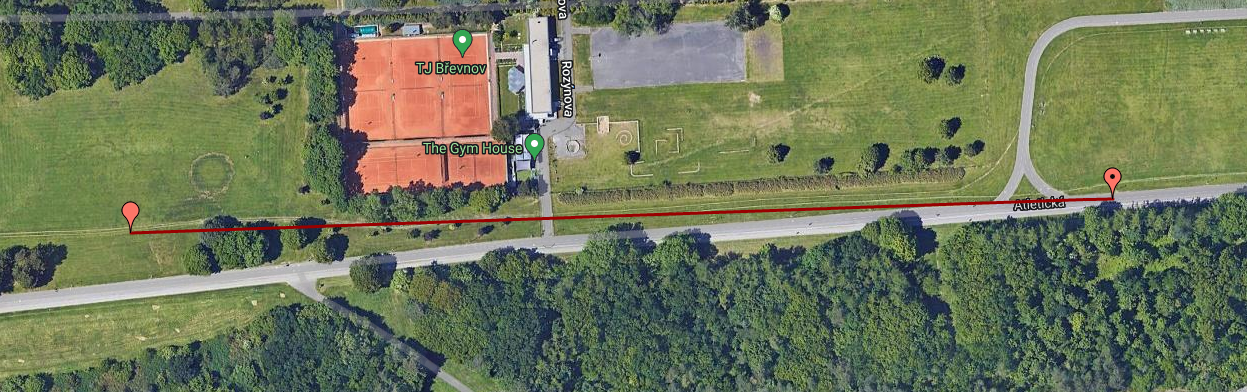
\includegraphics[width=0.9\linewidth]{fig/control_range.png}
\caption{Control distance}
\label{fig:control_range}
\end{figure}

GPS coordinates along with the calculated distance from the initial position are in table \ref{tab:gps_dist}. The measured control distance is visualized in figure \ref{fig:control_range}. 
\begin{table}[h]
   \renewcommand{\arraystretch}{1.1}
   \centering
    \caption{GPS coordinates and distances from the initial position}\label{tab:gps_dist}   
    \begin{tabular}{c c c}
       \noalign{\hrule height 1.1pt}\noalign{\smallskip}
	    & \bfseries GPS coordinates & \bfseries Calculated distance\\[0.2em]
	\noalign{\hrule height 1.1pt}\noalign{\smallskip}     
initial position		& 50.0792036N, 14.3716383E	& -- \\
occasional outages	& 50.0790850N, 14.3663733E	& \SI{375.9}{\m} \\
frequent outages		& 50.0793289N, 14.3631853E	& \SI{603.3}{\m} \\
signal 'lost'		& 50.0794572N, 14.3609497E	& \SI{763.2}{\m} \\
       \noalign{\smallskip}\noalign{\hrule height 1.1pt}
    \end{tabular}
\end{table} 